\documentclass[11pt,a4paper,oneside]{report}
\usepackage{iftex}
\ifPDFTeX
  \usepackage[utf8]{inputenc}
  \usepackage[T1]{fontenc}
  \usepackage{lmodern}
\else
  \usepackage{fontspec}
  \setmainfont{Latin Modern Roman}
  \setsansfont{Latin Modern Sans}
  \setmonofont{Latin Modern Mono}
\fi
\usepackage[spanish,es-tabla]{babel}
\usepackage[margin=2.5cm]{geometry}
\usepackage{graphicx}
\usepackage{booktabs,longtable,array}
\usepackage{xcolor}
\usepackage{listings}
\usepackage{enumitem}
\usepackage{tikz}
\usetikzlibrary{arrows.meta,positioning,shapes.geometric,babel}
\usepackage{hyperref}
\hypersetup{hypertexnames=false,colorlinks=true,linkcolor=blue!45!black,urlcolor=blue!55!black,citecolor=blue!45!black,
  pdftitle={Sistema de Gestión de Capacitaciones -- Paz Sur},pdfauthor={Equipo UNSAAC}}
\urlstyle{same}
\setlength{\parskip}{0.45em}
\setlength{\parindent}{0pt}
\setlist{itemsep=0.15em,topsep=0.3em}
\newcolumntype{P}[1]{>{\raggedright\arraybackslash}p{#1}}
\lstdefinelanguage{JavaScript}{
  morekeywords={import,from,export,const,let,return,if,else,throw,new,function,async,await,try,catch,finally,true,false,null},
  sensitive=true,
  morecomment=[l]{//},morecomment=[s]{/*}{*/},
  morestring=[b]',morestring=[b]"
}
\lstdefinestyle{codigo}{
  basicstyle=\ttfamily\footnotesize,
  keywordstyle=\color{blue!60!black},commentstyle=\color{green!35!black},
  stringstyle=\color{red!45!black},
  breaklines=true,breakatwhitespace=false,columns=fullflexible,
  keepspaces=true,showstringspaces=false,frame=single,
  numbers=left,numberstyle=\tiny\color{gray},numbersep=7pt,
  tabsize=2,captionpos=b,
  literate={á}{{\'a}}1 {é}{{\'e}}1 {í}{{\'i}}1 {ó}{{\'o}}1 {ú}{{\'u}}1
    {ñ}{{\~n}}1 {ü}{{\"u}}1 {Á}{{\'A}}1 {É}{{\'E}}1 {Í}{{\'I}}1
    {Ó}{{\'O}}1 {Ú}{{\'U}}1 {Ñ}{{\~N}}1 {¿}{{?`}}1 {¡}{{!`}}1
    {—}{{---}}1 {–}{{--}}1 {…}{{...}}1
}
\lstset{style=codigo}
\newcommand{\fuenteMermaid}[2]{%
  \section{#1}
  Fuente versionable: \path{docs/diagramas/#2}.
  \IfFileExists{../diagramas/#2}{%
    \lstinputlisting[language={},numbers=none]{../diagramas/#2}%
  }{%
    \IfFileExists{diagramas/#2}{%
      \lstinputlisting[language={},numbers=none]{diagramas/#2}%
    }{%
      \textbf{Fuente pendiente:} ejecutar el preparador de Overleaf.%
    }%
  }%
}
\newcommand{\pendiente}{\textbf{Pendiente de verificación.}}
\newcommand{\fragmentocodigo}[4]{%
  \IfFileExists{../../#1}{%
    \lstinputlisting[language=JavaScript,firstline=#2,lastline=#3,caption={#4}]{../../#1}%
  }{%
    \IfFileExists{codigo/#1}{%
      \lstinputlisting[language=JavaScript,firstline=#2,lastline=#3,caption={#4}]{codigo/#1}%
    }{%
      \textbf{Fragmento pendiente:} no se encontró \texttt{\detokenize{#1}}.
      Ejecutar el preparador de Overleaf sobre el repositorio completo.%
    }%
  }%
}
\begin{document}
\begin{titlepage}
  \centering
  {\Large\bfseries UNIVERSIDAD NACIONAL DE SAN ANTONIO ABAD DEL CUSCO\par}
  \vspace{0.6cm}
  {\large Facultad: por confirmar con el equipo\par}
  {\large Escuela profesional: denominación oficial por confirmar\par}
  \vspace{1cm}
  \IfFileExists{imagenes/escudo-unsaac.png}{%
    \includegraphics[width=3.2cm,height=3.8cm,keepaspectratio]{imagenes/escudo-unsaac.png}%
  }{%
    \fbox{\parbox[c][3.3cm][c]{4cm}{\centering Escudo UNSAAC\\[0.3cm]
      \small Incorporar archivo institucional autorizado en\\
      \path{imagenes/escudo-unsaac.png}}}%
  }
  \par
  \vspace{1cm}
  {\LARGE\bfseries Sistema de Gestión de Capacitaciones\par}
  \vspace{0.25cm}
  {\Large Paz Sur --- Cusco\par}
  \vspace{0.7cm}
  {\large Informe de Ingeniería de Software I\par}
  {\large Primer incremento y diseño del producto\par}
  \vspace{0.8cm}
  \begin{minipage}{0.92\textwidth}
    \textbf{Docente:} Jisbaj Gamarra Salas.\\[0.4cm]
    \textbf{Integrantes:}
    \begin{itemize}
      \item Brenda Lucia Mayhuire Chacón.
      \item Adel Alejandro Merma Ccarhuarupay.
      \item Franshesco (apellidos por confirmar).
      \item Daniela (apellidos por confirmar).
    \end{itemize}
    \textbf{Implementación:} asistida por Codex; revisión humana del incremento pendiente de registro.
  \end{minipage}
  \vfill
  {\large Cusco, Perú\par}
  {\large 12 de noviembre de 2026\par}
\end{titlepage}
\pagenumbering{roman}
\chapter*{Resumen}
\addcontentsline{toc}{chapter}{Resumen}
Este proyecto propone organizar la planificación y el seguimiento de las capacitaciones de la empresa comercial Paz Sur. El registro manual de asistencia y su eventual transcripción a hojas de cálculo dificultan la consulta y la verificación de información. El alcance candidato reúne 28 historias de usuario que deben contrastarse con el cliente.

El informe presenta un proceso iterativo, incremental y adaptativo, una arquitectura de monolito modular y el primer incremento de autenticación, usuarios, roles y planificación de capacitaciones. La base inspeccionada contenía documentación y no una aplicación ejecutable; por ello se conserva el contrato existente y se construye el incremento sin atribuirle una historia previa ficticia. La interfaz utiliza React y TypeScript; la API, Node.js y Express; la persistencia local, SQLite con migraciones. PostgreSQL es una opción de evolución pendiente de acordar.

Los resultados de ejecución se consignan en el capítulo de pruebas y en su tabla de evidencia. El diseño de participantes, sesiones, asistencia, resultados, reportes, certificados y catálogos no debe confundirse con funcionalidades terminadas. La revisión humana, la integración y la validación de reglas comerciales se registrarán cuando efectivamente ocurran.

\textbf{Palabras clave:} capacitación, requisitos, Scrum, Kanban, pruebas, arquitectura, UNSAAC.
\tableofcontents
\listoffigures
\listoftables
\clearpage
\pagenumbering{arabic}
\chapter{Introducción}
\section{Descripción del problema}
Paz Sur es una empresa comercial ubicada en Cusco, Perú. Según la información proporcionada por el equipo, sus trabajadores reciben capacitaciones internas y de marcas proveedoras. Algunas actividades se vinculan a temporadas comerciales, como campaña escolar, Navidad y Día de la Madre. El registro de asistencia se realiza parcialmente de forma manual y puede transcribirse después a Excel.

Este procedimiento requiere organizar la capacitación, identificar participantes y conservar un historial consultable. No se han confirmado cantidades de trabajadores, sedes, capacitaciones, costos, tiempos de transcripción ni tasas de error. Por tanto, el informe no atribuye cifras o problemas adicionales a la empresa.

\section{Objetivo general}
Desarrollar progresivamente un sistema de gestión de capacitaciones que permita organizar, consultar y verificar información, con implementación ejecutable, persistencia, controles de acceso, pruebas y documentación defendible por el equipo.

\section{Objetivos específicos}
\begin{enumerate}
  \item Inspeccionar el repositorio y separar hechos, supuestos y propuestas.
  \item Formular requisitos verificables y un backlog candidato trazable.
  \item Diseñar una arquitectura coherente con los recursos de cuatro estudiantes.
  \item Construir un primer flujo de extremo a extremo de acceso, usuarios, roles y capacitaciones.
  \item Ejecutar verificaciones disponibles y registrar resultados sin fabricar evidencia.
  \item Preparar el diseño y las prioridades de las iteraciones posteriores.
\end{enumerate}

\section{Alcance y límites del informe}
El primer incremento aborda HU-01, HU-02, HU-03, HU-04 y HU-16 como dependencia de autenticación. El diseño contempla las 28 historias; no se declara implementado todo ese alcance. Las reglas de asistencia, evaluaciones y certificados aún requieren validación. Un certificado puede existir en determinadas capacitaciones y no se presupone obligatorio.

Las versiones V1 a V4 expresan objetivos de evolución. No se crean etiquetas retroactivas para simular una secuencia histórica. El estado de terminado depende también de revisión humana e integración, además de pruebas locales.

\section{Organización del documento}
Los capítulos presentan contexto, proceso, requisitos, arquitectura, planificación, implementación, pruebas, evolución estructural y resultados. Los anexos conservan la bitácora y las fuentes Mermaid. Los fragmentos de código se importan de archivos reales del repositorio para reducir divergencias entre informe e implementación.

\chapter{Contexto y fundamento técnico}
\section{Participantes y responsabilidades}
El proyecto corresponde al curso Ingeniería de Software I de la UNSAAC, con el docente Jisbaj Gamarra Salas. El equipo está conformado por Brenda Lucia Mayhuire Chacón, Adel Alejandro Merma Ccarhuarupay, Franshesco y Daniela. No se completan apellidos, nombres institucionales de facultad o escuela, ni responsabilidades aceptadas mediante inferencias.

La coordinación propuesta debe acordar quién representa las decisiones del cliente, quién facilita el proceso y quién revisa cada entrega. La colaboración con IA no sustituye la responsabilidad de comprender y revisar el código. No se atribuye a un integrante una implementación manual o una aprobación que no haya realizado.

\section{Diagnóstico del repositorio}
La referencia inicial inspeccionada fue \texttt{cf6e720}, en la rama \texttt{main}. El árbol contenía README, el contrato de implementación y documentos de coordinación. No se encontraron la aplicación, un archivo de dependencias ni pruebas ejecutables en ese punto de partida.

Se observaron referencias remotas de integrantes: \path{origin/AD-1-registro-usuarios}, \path{origin/BrendaPro} y \path{origin/feature/brenda-mayhuire}. Su inspección no reveló una aplicación recuperable. Esta constatación no afirma que el código no exista en otras computadoras o referencias no disponibles.

Los documentos antiguos mencionan otra ruta local, una aplicación previa, SQLite y herramientas instaladas en esa otra situación. Se conservan como antecedentes y no como evidencia del entorno actual. La solicitud vigente autoriza construir el primer incremento; no se aplica automáticamente el antiguo límite de diagnóstico F0-01.

\section{Restricciones e incertidumbres}
\begin{itemize}
  \item Reglas comerciales incompletas y textos originales de Jira no contrastados.
  \item Capacidad académica de cuatro estudiantes sin velocidad histórica medida.
  \item Prohibición de push, merge, borrados masivos y publicaciones sin autorización.
  \item No utilizar credenciales reales ni datos personales de la empresa como datos de demostración.
  \item Motor PostgreSQL y servicios Supabase/Render mencionados como intención, pero sin conexión o migración verificadas.
  \item Compilador LaTeX no encontrado en el primer diagnóstico; una comprobación posterior localizó MiKTeX. La compilación se registra de forma separada de la preparación de fuentes.
\end{itemize}

\section{Fundamento teórico}
Un requisito funcional describe una capacidad observable, como registrar una capacitación; un requisito no funcional expresa una cualidad o restricción, como evitar que una cuenta sin permiso edite registros. Una arquitectura separa responsabilidades para permitir cambios y pruebas sin concentrar todo el comportamiento en una pantalla.

Un incremento debe aportar un resultado verificable. Una iteración ofrece la oportunidad de inspeccionar y ajustar el trabajo. La combinación permite aprender de un flujo pequeño antes de extenderlo. Scrum aporta un marco de inspección y adaptación con objetivos y artefactos \cite{scrum2020}. Kanban ayuda a definir y gestionar el flujo y sus límites \cite{kanban2025}. Las prácticas de XP orientadas a pruebas y refactorización se seleccionan cuando ayudan a mantener el diseño y el comportamiento \cite{xp}.

La trazabilidad conecta una necesidad con aceptación, código y verificación. No basta con que un nombre de historia aparezca en un archivo: se debe poder señalar la operación, los límites y el resultado comprobado.

\chapter{Proceso de desarrollo}
\section{Enfoque seleccionado}
Se propone un proceso iterativo, incremental y adaptativo. Cada Sprint de dos semanas debe tener un objetivo demostrable y un subconjunto de historias ajustado a la capacidad real. Scrum organiza la coordinación; Kanban hace visible el flujo; las prácticas técnicas de XP apoyan pruebas, refactorización e integración cuando existan las condiciones.

Esta es una adaptación para un trabajo académico, no una certificación de que ya se ejecutó Scrum. No se registran Daily Scrum, Sprint Review, retrospectivas, programación en pareja o TDD como actividades realizadas sin evidencia.

\section{Artefactos y eventos propuestos}
El Product Backlog mantiene el alcance candidato ordenado. El Sprint Backlog reúne el objetivo, historias seleccionadas y tareas. El incremento debe cumplir la Definition of Done acordada. Se propone una planificación inicial, un seguimiento breve y periódico, una revisión de producto y una retrospectiva al cierre; el equipo debe registrar fechas y resultados reales.

La guía detallada se conserva en \path{docs/PROCESO_DESARROLLO.md}. Los nombres de responsables propuestos no equivalen a una aceptación de sus funciones ni a una contribución ya realizada.

\section{Flujo y límites de trabajo}
Se plantea el tablero Pendiente, Lista, En curso, En revisión, Verificada y Hecha. Como política inicial para cuatro integrantes se recomienda una tarea de implementación activa por persona y un máximo de dos tareas en revisión. La coordinación puede reducir el WIP si aparecen bloqueos o archivos compartidos. Estos límites deben revisarse con observaciones del flujo, no tratarse como datos históricos.

Un bloqueo se anota con causa, responsable de resolverlo y siguiente acción. Si compromete el objetivo del Sprint se comunica al coordinador y se negocia alcance. No se declara terminada una tarea bloqueada por falta de acceso, revisión o integración.

\section{Definition of Done}
Una funcionalidad solo puede declararse terminada si cumple aceptación, valida entradas, persiste correctamente, aprueba las pruebas pertinentes, no tiene errores conocidos que impidan su flujo principal, cuenta con revisión humana registrada, está documentada y se integró en la rama acordada. La evidencia debe poder reproducirse.

Los criterios de una historia son específicos: por ejemplo, rechazar un correo duplicado. La DoD es transversal: por ejemplo, exigir revisión de código y documentación. Una batería local aprobada no satisface por sí sola todos los puntos de la DoD.

\section{Métricas y uso de IA}
Se proponen tiempo de ciclo, WIP, tareas bloqueadas, defectos encontrados y porcentaje de aceptación verificada. No se inventa velocidad de Sprints anteriores. La estimación de puntos es relativa y debe contrastarse con el equipo.

La plataforma identifica al agente como Codex basado en GPT-6; no expone aquí una variante exacta verificable. Se registra asistencia de IA sin atribuir autoría humana exclusiva. Las personas revisan requisitos, decisiones, código y evidencia. Los resultados de herramientas deben conservarse, y ningún texto generado sustituye una aprobación de Paz Sur.

\chapter{Requisitos y trazabilidad}
\section{Fuentes y estado de validación}
El prompt del proyecto aporta 28 historias de referencia. Estas constituyen el alcance candidato; su correspondencia con claves, textos, estimaciones y criterios reales de Jira sigue pendiente. No se reemplazan las estimaciones históricas de Jira con los puntos propuestos en la documentación.

Las fichas completas están en \path{docs/BACKLOG.md}; los criterios verificables y sus pruebas, en \path{docs/CRITERIOS_ACEPTACION.md}; requisitos y supuestos, en \path{docs/REQUISITOS.md}; y el vínculo con implementación y evidencia, en \path{docs/TRAZABILIDAD.md}.

\section{Catálogo de historias candidatas}
\begin{longtable}{P{1.5cm}P{8.1cm}P{3.1cm}}
\caption{Historias de referencia y alcance de implementación}\label{tab:historias}\\
\toprule ID & Nombre & Estado de alcance \\ \midrule
\endfirsthead
\toprule ID & Nombre & Estado de alcance \\ \midrule
\endhead
HU-01 & Registrar usuarios & Incluida en V1 \\
HU-02 & Asignar roles y permisos & Incluida en V1 \\
HU-03 & Registrar capacitación & Incluida en V1 \\
HU-04 & Modificar capacitación & Incluida en V1 \\
HU-05 & Asignar instructor & Candidata posterior \\
HU-06 & Registrar participantes & Candidata posterior \\
HU-07 & Consultar capacitaciones asignadas & Parcial: consulta por instructor V1 \\
HU-08 & Registrar asistencia & Candidata posterior \\
HU-09 & Registrar evaluaciones & Candidata posterior \\
HU-10 & Registrar certificado & Candidata posterior \\
HU-11 & Consultar capacitaciones inscritas & Candidata posterior \\
HU-12 & Consultar resultados & Candidata posterior \\
HU-13 & Consultar historial de capacitación & Candidata posterior \\
HU-14 & Consultar reportes consolidados & Candidata posterior \\
HU-15 & Consultar estado de las capacitaciones & Parcial: estado en V1 \\
HU-16 & Iniciar sesión & Dependencia incluida en V1 \\
HU-17 & Gestionar instructores & Candidata posterior \\
HU-18 & Descargar certificado & Candidata posterior \\
HU-19 & Gestionar cupos de capacitación & Parcial: capacidad en V1 \\
HU-20 & Registrar marcas proveedoras & Candidata posterior \\
HU-21 & Gestionar campañas comerciales & Candidata posterior \\
HU-22 & Gestionar trabajadores por sede y área & Candidata posterior \\
HU-23 & Consultar trabajadores pendientes & Candidata posterior \\
HU-24 & Consultar capacitaciones por marca & Candidata posterior \\
HU-25 & Consultar capacitaciones por sede & Candidata posterior \\
HU-26 & Recibir alertas de programación & Candidata posterior \\
HU-27 & Reprogramar capacitaciones pendientes & Parcial: edición en V1 \\
HU-28 & Registrar sesiones de capacitación & Candidata posterior \\
\bottomrule
\end{longtable}

Que una capacitación permita un instructor opcional, muestre estado o tenga capacidad no acredita el cierre de HU-05, HU-15, HU-19 o HU-27 completas. Es necesario contrastar los criterios de cada historia y demostrar todos sus casos.

\section{Las tres C e INVEST}
Cada historia se formula como tarjeta con rol, necesidad y beneficio; la conversación registra incertidumbres y alternativas; la confirmación establece criterios verificables. INVEST se usa para revisar independencia, posibilidad de negociación, valor, estimación, tamaño y capacidad de prueba.

Las dependencias reales no se ocultan para aparentar independencia absoluta. Por ejemplo, registrar asistencia requiere una sesión y una inscripción válidas. Historias grandes como reportes o gestión de trabajadores deben dividirse en entregas pequeñas una vez acordadas las consultas y reglas prioritarias.

\section{Ejemplo de aceptación}
Para HU-03, un usuario autorizado que envía código único, título, periodo válido y capacidad positiva debe obtener una capacitación persistida. Un periodo invertido, un cupo cero o un estado inicial finalizada se rechazan. El código duplicado debe producir un conflicto comprensible y no una segunda fila. Un participante no obtiene permiso de escritura por enviar una solicitud manual.

Estos casos son específicos de HU-03 y se complementan con la DoD general. El registro de su ejecución pertenece al capítulo de pruebas, no a la definición del requisito.

\section{Supuestos que requieren conversación}
Se deben confirmar roles y alcance de RR. HH./gerencia, trabajadores sin cuenta, sedes y áreas, transiciones y reapertura, forma de evaluación, umbrales de asistencia, emisión opcional de certificados, reprogramación y destinatarios de alertas. Las cifras 80\,\% y 14/20 provienen del contrato, no de una validación documentada con el cliente.

\chapter{Arquitectura y modelos}
\section{Monolito modular}
Se separan presentación, entrada HTTP, lógica de negocio y persistencia. Un solo proceso backend y un solo motor de datos simplifican el arranque y las pruebas. La decisión completa se documenta en \path{docs/ARQUITECTURA.md} y \path{docs/DECISIONES_TECNICAS.md}.

\begin{figure}[htbp]
\centering
\begin{tikzpicture}[
  bloque/.style={draw,rounded corners,align=center,minimum width=9.5cm,minimum height=0.95cm,fill=blue!5},
  >=Latex,node distance=0.7cm]
  \node[bloque] (ui) {Presentación: React + TypeScript\\Formularios y mensajes en español};
  \node[bloque,below=of ui] (http) {API: Express\\Sesión, CSRF, permisos, validación y respuestas};
  \node[bloque,below=of http] (servicios) {Servicios de aplicación\\Usuarios, roles y capacitación};
  \node[bloque,below=of servicios] (db) {Persistencia: SQLite\\Migraciones, claves foráneas y transacciones};
  \draw[->] (ui) -- node[right,font=\small] {HTTP/JSON} (http);
  \draw[->] (http) -- (servicios);
  \draw[->] (servicios) -- node[right,font=\small] {SQL parametrizado} (db);
\end{tikzpicture}
\caption{Arquitectura del primer incremento. No se representa un despliegue externo.}
\end{figure}

\section{Modelo de datos V1}
La base contiene usuarios, roles, permisos, asignaciones, sesiones de autenticación, capacitaciones, auditoría y control de migraciones. Una sesión de autenticación no es una sesión de capacitación: la primera mantiene el acceso; la segunda será una unidad académica en un incremento posterior.

Las tablas \texttt{user\_roles} y \texttt{role\_permissions} resuelven relaciones de muchos a muchos sin repetir listas de texto en una columna. El correo y el código de capacitación son únicos sin distinguir mayúsculas; el documento es opcional y único cuando existe. Una capacitación tiene responsable y puede tener instructor. El cupo admite de 1 a 10\,000 personas.

Las migraciones se registran y aplican transaccionalmente. Los roles y permisos iniciales se cargan solo durante la primera migración; abrir la base o añadir otra migración no sobreescribe las personalizaciones administrativas. Los timestamps técnicos usan UTC y el panel determina el día actual en \texttt{America/Lima}.

\begin{table}[htbp]
\centering
\caption{Relaciones principales del modelo físico V1}
\begin{tabular}{P{5.2cm}P{6.8cm}}
\toprule Relación & Integridad \\ \midrule
Usuario--rol & PK compuesta impide asignación duplicada \\
Rol--permiso & FK a catálogos conocidos y combinación única \\
Usuario--sesión de acceso & Token hasheado, vencimiento y usuario válido \\
Usuario--capacitación & Responsable obligatorio; instructor opcional \\
Usuario--auditoría & Actor de una acción, sin contraseñas o cookies \\
\bottomrule
\end{tabular}
\end{table}

\section{Modelo candidato del producto}
El diseño posterior contempla trabajador, sede, área, marca proveedora, campaña, sesión académica, inscripción, asistencia, evaluación, certificado y notificación. No se crean entidades por acumular nombres: un instructor V1 es un usuario con rol instructor, sin duplicar su identidad en una tabla independiente.

Cada inscripción futura vincula persona y capacitación, con unicidad de esa pareja. Cada marca de asistencia vincula inscripción y sesión y debe comprobar que ambas pertenecen a la misma capacitación. Evaluación y certificado son opcionales por inscripción. Las alertas se plantean dentro de la aplicación; no se asume un proveedor de correo o SMS.

La alternativa candidata del contrato exige una cuenta para inscribirse, aunque un perfil de trabajador pueda existir sin acceso. Si se requiere inscribir a trabajadores sin cuenta, la FK deberá apuntar al trabajador y se revisarán contrato, permisos y migración antes de implementar. El diagrama señala esta incertidumbre en lugar de simular una solución aprobada.

\section{Flujo de estados}
\begin{figure}[htbp]
\centering
\begin{tikzpicture}[
  estado/.style={draw,rounded corners,align=center,minimum height=0.8cm,minimum width=2.5cm,fill=blue!5},
  >=Latex,node distance=1cm]
  \node[estado] (p) {Planificada};
  \node[estado,right=of p] (s) {Programada};
  \node[estado,right=of s] (c) {En curso};
  \node[estado,below=of c] (f) {Finalizada};
  \node[estado,below=of s] (x) {Cancelada};
  \draw[->] (p) to[bend left=12] (s);
  \draw[->] (s) to[bend left=12] (p);
  \draw[->] (s) -- (c);
  \draw[->] (c) -- (f);
  \draw[->] (p) -- (x);
  \draw[->] (s) -- (x);
  \draw[->] (c) -- (x);
\end{tikzpicture}
\caption{Transiciones provisionales V1. Finalizada y cancelada son inmutables.}
\end{figure}

La creación admite planificada o programada. La edición puede conservar un estado abierto. No se permite saltar directamente de planificada a finalizada. La reapertura no forma parte de este incremento y requiere una decisión del cliente.

\section{Permisos y seguridad}
La API comprueba permisos en el servidor y filtra los datos por alcance. Los seis roles iniciales son administrador, coordinador, instructor, participante, RR. HH. y gerencia. El administrador tiene todas las capacidades y su rol se protege; los demás roles parten de la matriz del contrato y sus permisos pueden editarse con autorización.

Asignar roles requiere \texttt{roles.manage}. Una cuenta delegada con solo \texttt{users.manage} crea únicamente participantes y no edita cuentas que tengan privilegios \texttt{users.manage} o \texttt{roles.manage}. El permiso \texttt{people.manage} habilita en V1 consultas reducidas para selectores, sin correo, documento, roles o permisos ajenos; las mutaciones de gestión de instructores y participantes continúan pendientes.

La contraseña se protege con \texttt{scrypt} y una sal propia; el navegador recibe una cookie HttpOnly con token opaco y la base almacena su hash. La sesión vence en ocho horas y se revoca al desactivar la cuenta o cambiar la contraseña. Las mutaciones requieren un token CSRF. Se limitan diez intentos de login por IP en quince minutos, incluidos los correctos y sin reiniciar contador al acertar. El control reside en memoria de una sola instancia y se pierde al reiniciar.

La explicación de estas primitivas se apoya en la documentación de Node \cite{nodecrypto} y las recomendaciones de OWASP \cite{owaspcsrf}. Un despliegue real requiere TLS, cookie Secure y revisar sus condiciones de operación.

\section{Patrones evaluados}
Strategy no se aplica todavía porque no hay varias políticas de evaluación aprobadas. Adapter se reconsiderará cuando exista un proveedor externo o una diferencia real de integración. Un mapa central de transiciones resuelve los estados V1 sin una jerarquía de clases State. Se documentan las condiciones de aplicación sin fabricar un problema para justificar un patrón.

El diagrama de clases del anexo representa responsabilidades conceptuales de módulos. La implementación backend utiliza funciones; no se afirma que esas clases existan literalmente en JavaScript.

\chapter{Planificación del primer incremento}
\section{Referencia histórica y propuesta actual}
La referencia histórica proporcionada por el usuario sitúa HU-01 a HU-04 en Sprint 1. No se han consultado las estimaciones originales de Jira y no se modifican. HU-16 se identifica como dependencia técnica y funcional del acceso protegido, sin afirmar que estuviera incluida históricamente.

La planificación propuesta se conserva en \path{docs/SPRINT_1.md}. La duración es dos semanas, pero no se inventan fechas de eventos, horas disponibles o velocidad del equipo. Antes de comprometer todo el alcance se deben contrastar disponibilidad, dificultad y criterios con los cuatro integrantes.

\section{Objetivo verificable}
Una cuenta administradora de demostración puede iniciar sesión, registrar una cuenta con un rol permitido, crear una capacitación, editarla y volver a consultar los datos persistidos. Las solicitudes sin acceso, los datos inválidos y los conflictos reciben errores comprensibles; el navegador no simula un guardado local.

\begin{table}[htbp]
\centering
\caption{Paquetes de trabajo del primer incremento}
\begin{tabular}{P{2cm}P{7cm}P{3cm}}
\toprule Referencia & Resultado esperado & Verificación \\ \midrule
HU-16 & Login, sesión vigente y logout & API y revisión de navegador \\
HU-01 & Alta, consulta y edición de usuarios & Validez, duplicado y acceso \\
HU-02 & Roles, asignaciones y permisos & Privilegios y administrador protegido \\
HU-03 & Crear capacitación persistente & Caso válido y límites \\
HU-04 & Editar sin violar integridad & Consulta posterior y estados \\
Técnica & Migraciones, semilla, documentación & Arranque reproducible \\
\bottomrule
\end{tabular}
\end{table}

\section{Entrega mínima y capacidad}
Si no existe capacidad para terminar todo en el Sprint, la entrega mínima debe contener login, un usuario autorizado y creación/consulta persistente de capacitación, con aceptación y pruebas. Edición completa de permisos u otras tareas deben registrarse pendientes, sin declarar terminado un incremento que no cumple su objetivo.

La documentación puede elaborarse en paralelo con límites de archivos claros, pero una revisión de código por otro integrante sigue siendo necesaria. Las tareas compartidas deben integrarse de forma consciente; las contribuciones de IA no representan automáticamente trabajo de cada estudiante.

\section{Evolución propuesta}
V2 revisará el diseño real y ampliará instructores y participantes cuando sus dependencias estén listas. V3 podrá incorporar sesiones, asistencia, historial y evaluaciones. V4 priorizará integración, seguridad, experiencia y funcionalidades restantes acordadas. Ninguna de estas metas se etiqueta como versión ya construida o probada.

\chapter{Implementación del primer incremento}
\section{Lenguajes y herramientas}
La interfaz utiliza TypeScript con React. La API utiliza JavaScript ESM ejecutado con Node.js 24 y Express 5. Zod valida entradas con mensajes en español; SQLite persiste datos mediante el módulo \texttt{node:sqlite}; Node Test Runner y Supertest verifican la API, y Playwright automatiza flujos de navegador Chrome.

Las versiones resueltas en esta construcción son Express 5.3.0, React 19.3.1, Zod 4.6.7, Vite 8.3.8 y TypeScript 7.0.2. La fuente reproducible es \path{package-lock.json}; estas versiones no estaban presentes en la base documental inicial. El entorno inspeccionado ofrece Node 24.16.0. La documentación oficial describe los requisitos y las funciones de Express, Vite y SQLite \cite{express5,vite,nodesqlite}.

\section{Archivos y comunicación entre módulos}
\begin{longtable}{P{5.7cm}P{7cm}}
\caption{Responsabilidades de archivos principales}\\
\toprule Archivo o carpeta & Responsabilidad \\ \midrule
\endfirsthead
\toprule Archivo o carpeta & Responsabilidad \\ \midrule
\endhead
\path{src/App.tsx} y módulos de interfaz & Formularios y vistas de acceso, panel, usuarios, roles y capacitaciones \\
\path{src/api.ts} & Solicitudes a la API y tratamiento de errores de contrato \\
\path{server/index.js} & Inicio del proceso y configuración del entorno \\
\path{server/app.js} & Composición de middleware, rutas y manejo final de errores \\
\path{server/routes/auth.js} & Inicio, consulta y cierre de sesión \\
\path{server/routes/users.js} & Entradas HTTP de usuarios y roles \\
\path{server/routes/trainings.js} & Entradas HTTP de capacitaciones y consultas iniciales \\
\path{server/services/user-service.js} & Reglas de usuarios, roles e integridad administrativa \\
\path{server/services/training-service.js} & Validación de planificación y transiciones \\
\path{server/security.js} & Hashing, sesiones, CSRF y autorización \\
\path{server/db.js} & Conexión, migraciones y transacciones \\
\path{server/migrations/001_initial.sql} & Esquema inicial con restricciones persistentes \\
\path{server/seed.js} & Datos ficticios de demostración y configuración de cuenta inicial \\
\path{tests/api.test.js} & Casos HTTP de usuarios, roles y capacitaciones \\
\path{tests/security.test.js} & Sesión, CSRF, límites y controles de privilegios \\
\path{tests/persistence.test.js} & Reapertura de base, rollback y migraciones incrementales \\
\path{tests/ui.spec.ts} & Flujos de navegador automatizados; resultados separados de API \\
\bottomrule
\end{longtable}

El formulario no ejecuta SQL. Envía JSON a una ruta, que valida y delega al servicio. El servicio aplica reglas y coordina persistencia. La respuesta informa éxito después de confirmar la operación. Una falla de integridad no debe dejar la auditoría o una asignación de rol parcialmente guardadas.

\section{Autenticación, usuarios y roles}
HU-16 habilita el flujo protegido de HU-01 y HU-02. El login verifica la contraseña y el estado activo; la cookie de sesión y el token CSRF acompañan solicitudes posteriores. Un usuario autenticado no recibe automáticamente permiso administrativo.

El registro de usuario admite nombres, apellidos, correo, documento opcional, área textual, especialidad, estado y roles. La contraseña solo es obligatoria al crear y nunca se devuelve en consultas. Una edición debe conservar administración activa y rechazar duplicados. La asignación de roles exige \texttt{roles.manage}; delegar solo \texttt{users.manage} no permite crear cuentas privilegiadas ni editar las que tengan gestión de usuarios o roles. La gestión de roles permite consultar el catálogo y cambiar permisos de roles no administrativos con autorización.

\section{Registro y edición de capacitaciones}
HU-03 y HU-04 usan una capacitación con código, título, descripción, periodo, horario, modalidad, ubicación, capacidad y estado. El responsable procede de la sesión autenticada; no se confía en un identificador privilegiado enviado por el navegador. El instructor es opcional y, cuando se informa, debe ser un usuario válido con el rol correspondiente.

La lista permite consulta y filtros. La creación admite estados iniciales definidos y la edición comprueba el grafo de transiciones. El control de capacidad V1 valida un entero entre 1 y 10\,000; aún no prueba un flujo de ocupación de cupos con inscripciones, porque ese módulo está pendiente. El instructor consulta únicamente capacitaciones asignadas. El participante no recibe filas ajenas mientras no exista el módulo de inscripciones.

\section{Fragmentos del código real}
Los siguientes listados se leen directamente del código del repositorio. Si se prepara una copia autónoma para Overleaf, el script incluido copia esos mismos archivos y registra sus hashes. No se presenta pseudocódigo como una captura de implementación.

\fragmentocodigo{server/db.js}{1}{45}{Inicio del módulo real de persistencia y migraciones}
\fragmentocodigo{server/security.js}{1}{55}{Inicio del módulo real de seguridad}
\fragmentocodigo{server/services/training-service.js}{1}{60}{Inicio del servicio real de capacitaciones}

\section{Ejecución reproducible}
Desde la raíz del proyecto, se instala con \texttt{npm.cmd ci}, se prepara \path{.env} desde \path{.env.example} y se definen credenciales ficticias propias para la demostración. Los valores reales no se incluyen en este informe. Después se aplican migraciones, se carga la semilla y se ejecuta el desarrollo:

\begin{lstlisting}[language={},numbers=none]
npm.cmd run db:migrate
npm.cmd run db:seed
npm.cmd run dev
\end{lstlisting}

La dirección y las variables exactas se consultan en el README y en el archivo de ejemplo que acompaña al incremento. Para comprobar tipos, API y compilación:

\begin{lstlisting}[language={},numbers=none]
npm.cmd run typecheck
npm.cmd test
npm.cmd run build
\end{lstlisting}

La prueba automatizada de interfaz requiere Chrome disponible y una compilación previa. Se ejecuta con \texttt{npm.cmd run test:ui}; su configuración inicia un servidor propio y una base ficticia aislada en el puerto 3101. No usa la base de demostración del usuario. Los resultados y las capturas reales, cuando se produzcan, se registran como evidencia separada.

El resultado observable esperado es iniciar sesión, guardar un usuario o una capacitación y recuperarlos de la API después de recargar. La prueba de persistencia en disco requiere volver a abrir la misma base; la presencia de una lista en pantalla por sí sola no demuestra ese comportamiento.

\section{Dificultades y pendientes}
Las guías iniciales no coincidían con el árbol real. Se decidió preservar los documentos y explicitar el nuevo punto de partida. Durante el trabajo se detectó falta de espacio en la unidad del perfil de usuario; las herramientas y el cache de instalación se dirigieron al espacio disponible del proyecto cuando fue necesario. Esto es una limitación del entorno y no una función del producto.

Los módulos de inscripción, asistencia, evaluación, historial, certificados, reportes consolidados, marcas, campañas, sedes y alertas quedan fuera del flujo principal V1. No se incorporan botones que aparenten guardar esas funciones.

\section{Interfaz verificada en navegador}
Las figuras se obtuvieron con Chrome y Playwright ejecutando la aplicación y su API aislada con datos ficticios. Son capturas reales del incremento; no representan aprobación del cliente ni revisión humana del equipo. Se comprobó también el guardado mediante formularios, el rechazo de correos duplicados y la consulta del detalle actualizado.
\begin{figure}[htbp]
  \centering
  \IfFileExists{../evidencias/v1-escritorio.png}{\includegraphics[width=\linewidth]{../evidencias/v1-escritorio.png}}{\IfFileExists{imagenes/v1-escritorio.png}{\includegraphics[width=\linewidth]{imagenes/v1-escritorio.png}}{Captura de escritorio no disponible en esta copia.}}
  \caption{Panel real de demostración en escritorio.}
\end{figure}
\begin{figure}[htbp]
  \centering
  \IfFileExists{../evidencias/v1-movil.png}{\includegraphics[height=14cm,keepaspectratio]{../evidencias/v1-movil.png}}{\IfFileExists{imagenes/v1-movil.png}{\includegraphics[height=14cm,keepaspectratio]{imagenes/v1-movil.png}}{Captura móvil no disponible en esta copia.}}
  \caption{Panel real de demostración en un viewport móvil.}
\end{figure}

\chapter{Pruebas y evidencia}
\section{Estrategia}
Se verifica la API real con Supertest y Node Test Runner. Los archivos \path{tests/api.test.js}, \path{tests/security.test.js} y \path{tests/persistence.test.js} utilizan bases aisladas y datos ficticios. Los casos cubren solicitudes válidas, entradas inválidas, límites y controles de acceso. Las consultas posteriores comprueban que la respuesta de éxito corresponde a datos guardados.

Playwright añade los flujos de \path{tests/ui.spec.ts} sobre Chrome y un servidor con base E2E propia. Es una automatización de navegador y no una revisión humana. Su ejecución se registra separadamente en la tabla de evidencia; escribir el archivo de prueba no demuestra que haya aprobado.

La documentación de aceptación define el resultado esperado; este capítulo registra lo observado. La definición de un caso no demuestra que haya sido ejecutado. Un análisis de tipos o una compilación frontend tampoco reemplazan pruebas de integración.

\section{Casos prioritarios}
\begin{longtable}{P{2.2cm}P{7.7cm}P{2.4cm}}
\caption{Cobertura que debe verificarse para el incremento}\\
\toprule Área & Caso y resultado esperado & Relación \\ \midrule
\endfirsthead
\toprule Área & Caso y resultado esperado & Relación \\ \midrule
\endhead
Acceso & Credenciales válidas crean sesión; contraseña inválida y cuenta inactiva se rechazan & HU-16 \\
Sesión & Sin cookie no se accede a rutas protegidas; logout invalida la sesión & HU-16 \\
CSRF & Una mutación autenticada sin token válido se rechaza & Seguridad \\
Usuarios & Alta válida y lectura posterior; duplicado de correo o documento rechazado & HU-01 \\
Roles & Asignar roles exige roles.manage; users.manage delegado no eleva privilegios ni edita cuentas administrativas & HU-02 \\
Capacitación & Registro válido, consulta y modificación persistidas & HU-03/04 \\
Límites & Capacidad cero, fecha invertida, hora inválida y datos incompletos se rechazan & HU-03/04 \\
Estado & Transición válida admitida; salto no permitido y edición de cierre rechazados & HU-04 \\
Alcance & Instructor no consulta capacitaciones ajenas; participante no ve datos de otros & Acceso a datos \\
Persistencia & Reapertura conserva registros; rollback revierte todo; migración incremental conserva catálogos personalizados & Técnica \\
\bottomrule
\end{longtable}

Los nombres y el número exacto de pruebas son los de los archivos y la salida del comando real. La tabla anterior no los sustituye ni promete cobertura de funcionalidades pendientes.

\section{Registro de ejecución}
% Actualizar exclusivamente con comandos y resultados realmente observados.
% Resultados locales reales. No equivalen a aprobación humana o CI remota.
\begin{longtable}{P{4.2cm}P{8.2cm}}
\caption{Evidencia de la sesión del 12 de noviembre de 2026}\label{tab:evidencia}\\
\toprule Comprobación & Resultado registrado \\ \midrule
\endfirsthead
\toprule Comprobación & Resultado registrado \\ \midrule
\endhead
Inspección Git & Base \texttt{cf6e720}; rama local de incremento \texttt{feature/v1-base-funcional}. Sin commit, push, merge o tag de esta entrega acreditados. \\
Motor local & Node 24.16.0; apertura de SQLite en memoria devolvió versión 3.53.0. \\
Instalación & 133 paquetes auditados después de incorporar Playwright; cero vulnerabilidades reportadas por npm en esa consulta. No equivale a una auditoría de seguridad. \\
\texttt{npm.cmd run check} & Verificación final: 28 pruebas aprobadas, 0 fallidas en 12.52 s; también análisis de tipos y build aprobados. Incluye fecha Lima y privilegios indirectos. Véase \path{docs/PRUEBAS.md}. \\
Tipos TypeScript & \texttt{tsc --noEmit} aprobado como paso de build. No se afirma ejecución separada del script typecheck. \\
\texttt{npm.cmd run build} & Aprobado con Vite 8.3.8, 22 módulos. El primer intento detectó falta de tipos del import CSS, corregida antes de la ejecución aprobada. \\
Prueba de navegador & Playwright y Chrome: 4 aprobadas, 0 fallidas en 9.0 s. Login/logout, alta/edición/duplicado de usuario, alta/edición/detalle de capacitación y panel móvil. Se corrigieron títulos que se cortaban en 390 px. Capturas reales en \path{docs/evidencias/}. \\
Compilación LaTeX & XeLaTeX falló por ausencia de xelatex.fmt. pdfLaTeX y BibTeX generaron el PDF tras corregir Babel/TikZ y usar fuentes Latin Modern. La inspección visual final se registra en \path{docs/PRUEBAS.md}. \\
Revisión humana e integración & PENDIENTES; no declarar cumplida la DoD completa sin estos registros. \\
\bottomrule
\end{longtable}


\section{Prueba manual propuesta}
Con la semilla ficticia y la aplicación ejecutándose, el revisor puede iniciar sesión, crear un usuario, intentar repetir su correo, crear una capacitación, editar su título y volver a consultar. Debe observar guardado real y errores comprensibles. Luego puede comprobar que una cuenta sin privilegios no dispone de las mismas acciones ni obtiene acceso mediante llamadas directas.

Esta secuencia es un protocolo pendiente hasta que una persona registre fecha, cuenta ficticia usada, resultado y observaciones. No se atribuye una ejecución de navegador a los cuatro integrantes ni se presentan capturas generadas como evidencia.

\section{Límites de la verificación}
Las pruebas de API y los flujos de navegador seleccionados no demuestran por sí solos accesibilidad completa, comportamiento en todos los dispositivos, concurrencia de producción o ausencia de vulnerabilidades. La revisión visual del frontend y la revisión del PDF se registran separadamente. La ejecución de una futura CI debe enlazarse a un resultado real del repositorio.

\chapter{Estructura, mantenimiento y refactorización}
\section{Situación inicial real}
En la referencia inicial no había implementación ejecutable que refactorizar. Por ello no se fabrica un listado anterior, un defecto histórico, una versión V2 ni una prueba de regresión sobre código ausente. La separación de rutas y servicios durante esta construcción es una decisión del primer incremento.

\section{Problema que se busca evitar}
Si un controlador mezclara validación HTTP, reglas de acceso, transiciones y SQL, sería difícil probar una regla sin simular toda la solicitud y difícil cambiar el acceso a datos. La arquitectura reduce ese riesgo con módulos explícitos. Esta motivación no constituye evidencia de que ese controlador monolítico haya existido en el repositorio.

La conexión se recibe por inyección; los servicios contienen las reglas; las rutas traducen solicitudes y respuestas. No se introduce una jerarquía de clases por preferencia. La cohesión se evalúa por responsabilidades y consumidores, no por el número de archivos.

\section{Protocolo para una refactorización futura}
Una tarea de V2 deberá registrar:
\begin{enumerate}
  \item Problema observado, archivo, función y referencia Git real.
  \item Comportamiento que debe conservarse y pruebas ejecutadas antes del cambio.
  \item Fragmento anterior obtenido de la referencia preservada, no reconstruido de memoria.
  \item Cambio concreto, principio o patrón pertinente y razón para elegirlo.
  \item Fragmento refactorizado y pruebas de regresión posteriores.
  \item Resultado, limitaciones y revisión humana efectivamente registrada.
\end{enumerate}

Si se añade una capacidad, como notificaciones por inscripción, se clasifica como ampliación funcional; no como refactorización pura. Los eventos de éxito deben ocurrir después del commit y solo se justifican si existe un consumidor real.

\section{Strategy, Adapter y evolución}
Strategy puede tener sentido si el cliente confirma diferentes algoritmos de evaluación o certificación. Adapter puede aislar una integración de proveedor externo. Ninguno se implementa solo para mostrarlo en el informe. La eventual migración PostgreSQL exige cambios comprobados y no se resuelve mediante una interfaz vacía.

La prioridad de mantenimiento es corregir defectos reales al encontrarlos. No se preserva un error deliberadamente para producir una historia académica de mejora.

\chapter{Resultados y limitaciones}
\section{Artefactos preparados}
La sesión construye el primer incremento local y el conjunto documental: diagnóstico, requisitos, backlog de 28 historias, criterios de aceptación, trazabilidad, proceso, planificación, decisiones, diagramas y fuentes del informe. El alcance funcional de implementación se concentra en autenticación, usuarios, roles y capacitaciones.

La evidencia de ejecución se lee en la tabla~\ref{tab:evidencia}. Un archivo creado, una ruta escrita o un botón visible no prueban por sí solos que el flujo esté verificado. Los resultados finales deben indicar los comandos efectivamente completados y sus limitaciones.

\section{Resultado esperado del flujo V1}
El administrador de demostración puede trabajar con cuentas ficticias y capacitaciones almacenadas en SQLite a través de una API protegida. La interfaz presenta carga, confirmación y error según la respuesta real. El acceso y la edición dependen de los permisos actuales, no de un rol escrito manualmente en el navegador.

Se preservan las ramas de integrantes y los documentos previos. No se presenta la construcción local como una integración, publicación, revisión de compañeros o aprobación de Paz Sur. No se crean tags V1--V4 para simular una evolución que no ocurrió.

\section{Limitaciones del producto}
\begin{itemize}
  \item No están implementados los flujos completos de participantes, asistencia, sesiones, resultados o historial.
  \item No se emiten certificados, ni se presupone que todas las capacitaciones los necesitan.
  \item Los catálogos de marcas, campañas, sedes y áreas son diseño candidato.
  \item Los reportes consolidados y las alertas no se presentan como disponibles por existir un permiso de catálogo.
  \item La matriz de roles, estados y reglas académicas necesita validación con el cliente.
  \item No se ha demostrado capacidad de producción, alta disponibilidad o cumplimiento normativo específico.
\end{itemize}

\section{Limitaciones del entorno y del proceso}
La falta de espacio en la unidad del perfil complicó la ejecución de herramientas. Se verificó disponibilidad de Node y SQLite. XeLaTeX se ejecutó realmente con instalación automática deshabilitada y falló por ausencia de \texttt{xelatex.fmt}; no pudo completar la generación del formato. Se preparó la alternativa pdfLaTeX con fuentes Latin Modern vectoriales y se corrigió la interacción entre Babel español y TikZ. El resultado de esa compilación se consigna en la tabla de evidencia, separado de la revisión visual del PDF.

Los Mermaid se revisaron como fuentes, pero su renderizado con un motor Mermaid no está verificado. El informe incluye esas fuentes y dos diagramas nativos TikZ; ambos tipos de artefacto deben distinguirse al presentar resultados.

Las ceremonias Scrum, las revisiones de compañeros y la integración en Git permanecen propuestas o pendientes hasta que existan registros. Las estimaciones de capacidad son propuestas y no reemplazan datos históricos de Jira.

\section{Siguiente actividad recomendada}
El equipo debe revisar el diff y ejecutar la demostración con datos ficticios, validar las reglas del primer incremento y registrar las observaciones. Después podrá seleccionar una tarea pequeña de participantes o instructores, verificar sus dependencias y completar sus criterios sin comprometer automáticamente el resto del producto.

\chapter{Conclusiones}
El desarrollo debe comenzar con un diagnóstico del árbol real. Los documentos previos aportaron un contrato útil, pero no demostraron la presencia de una aplicación en este clon. Preservar esa distinción permitió construir el primer incremento sin borrar el trabajo del equipo ni atribuirle evidencia inexistente.

La arquitectura de monolito modular separa interfaz, HTTP, reglas y persistencia con complejidad razonable para cuatro estudiantes. SQLite facilita la demostración local; PostgreSQL sigue siendo una decisión de evolución que requiere migración y pruebas reales.

El enfoque iterativo, incremental y adaptativo permite verificar un flujo pequeño antes de ampliar el alcance. Scrum, Kanban y prácticas de XP ofrecen una propuesta de trabajo; su aplicación efectiva requiere registros y responsabilidad humana.

La documentación de 28 historias no equivale a su implementación. La aceptación de cada historia, las verificaciones ejecutadas, la revisión de código y la integración determinan si un incremento cumple la Definition of Done.

El informe conserva decisiones, modelos, limitaciones y fragmentos importados del código. Debe actualizarse con cada módulo importante y con las pruebas realmente realizadas. La siguiente iteración debe partir del incremento revisado y de reglas comerciales confirmadas.

\bibliographystyle{plain}
\bibliography{referencias}
\appendix
\chapter{Bitácora de desarrollo}
\begin{longtable}{P{2.2cm}P{2.6cm}P{7.5cm}}
\caption{Actividades documentadas en esta sesión}\\
\toprule Fecha Lima & Módulo & Actividad, motivo y resultado \\ \midrule
\endfirsthead
\toprule Fecha Lima & Módulo & Actividad, motivo y resultado \\ \midrule
\endhead
2026-11-12 & Diagnóstico & Inspección del árbol y referencias Git. Base \texttt{cf6e720} con documentación y sin aplicación. Se preservan los antecedentes y se distingue otra carpeta descrita por los TXT. \\
2026-11-12 & Arquitectura & Elaboración de \path{docs/ARQUITECTURA.md}, registro ADR y 11 fuentes Mermaid. Se diferencian nueve tablas V1 del modelo académico candidato. \\
2026-11-12 & Planificación & Construcción de documentos de requisitos, aceptación, backlog, trazabilidad y proceso por el equipo de agentes. Sus estimaciones y responsabilidades propuestas no se atribuyen a aprobación humana. \\
2026-11-12 & V1 & Construcción asistida por IA de API, persistencia e interfaz de HU-01 a HU-04 y HU-16. Los archivos reales se detallan en el capítulo de implementación; las pruebas finales se registran en la tabla de evidencia. \\
2026-11-12 & Entorno & Detección de falta de espacio en la unidad del perfil. El agente principal informó instalación de dependencias completada en el espacio disponible. Node 24.16.0 y SQLite 3.53.0 comprobados. \\
2026-11-12 & Informe & Creación de \path{main.tex}, once capítulos, bibliografía y anexos. Escudo, facultad/escuela y nombres incompletos se dejan preparados para confirmación. No se inventa una imagen institucional. \\
2026-11-12 & Calidad & Ejecución final de API, tipos, build y compilación LaTeX: ver tabla de evidencia, que debe actualizarse con resultados reales. Revisión humana e integración pendientes. \\
2026-11-12 & Regresión final & \texttt{npm.cmd run check}: 28 pruebas aprobadas y build aprobado; Playwright: 4 pruebas Chrome aprobadas. Se corrigieron escalamiento directo e indirecto, migraciones incrementales, fecha Lima, límite de login y títulos móviles. \\
2026-11-12 & Informe final & XeLaTeX no generó formato; pdfLaTeX con BibTeX compiló 50 páginas tras corregir Babel/TikZ, fuentes y portada. Capturas reales incluidas; revisión visual mediante páginas PNG y hojas de contacto. No se publicaron cambios. \\
2026-11-12 & Alineación & Actualizados arquitectura, ADR y capítulos con permisos delegados, revocación, límite de login, migración idempotente y archivos de pruebas reales. Se diferencia consulta de instructores V1 de gestión futura. \\
2026-11-12 & Compilación & XeLaTeX falló por formato ausente. En \path{main.tex} se añadió compatibilidad Babel--TikZ, anclas PDF no duplicadas y fuentes Latin Modern para el intento pdfLaTeX. El resultado final y la revisión visual se registran por separado. \\
\bottomrule
\end{longtable}

\section{Registro de futuras entradas}
Cada entrada posterior debe indicar fecha, historia o tarea, archivos modificados, motivo, dificultad, comandos ejecutados, resultado, evidencia, revisión humana y pendiente. Cuando exista una refactorización, se conservarán referencias reales del antes y después y las pruebas correspondientes.

Este registro describe asistencia de IA. No asigna a Brenda, Adel, Franshesco o Daniela pruebas, escritura manual, ceremonias o revisiones que no hayan confirmado.

\chapter{Fuentes de los diagramas}
Las fuentes distinguen V1 del diseño futuro. Los diagramas de inscripción y asistencia son modelos candidatos y no evidencia de endpoints ejecutados.
\fuenteMermaid{Arquitectura general}{arquitectura.mmd}
\fuenteMermaid{Casos de uso}{casos_uso.mmd}
\fuenteMermaid{Entidad--relación V1}{er_v1.mmd}
\fuenteMermaid{Entidad--relación del producto candidato}{er_producto_candidato.mmd}
\fuenteMermaid{Responsabilidades de módulos}{clases.mmd}
\fuenteMermaid{Componentes}{componentes.mmd}
\fuenteMermaid{Registrar una capacitación}{secuencia_registrar_capacitacion.mmd}
\fuenteMermaid{Inscribir un participante: diseño futuro}{secuencia_inscribir_participante.mmd}
\fuenteMermaid{Registrar asistencia: diseño futuro}{secuencia_registrar_asistencia.mmd}
\fuenteMermaid{Estados}{estados.mmd}
\fuenteMermaid{Roles y permisos}{roles_permisos.mmd}
\end{document}
